\documentclass[conference]{IEEEtran}
\IEEEoverridecommandlockouts

\usepackage{cite}
\usepackage{amsmath,amssymb,amsfonts}
\usepackage{algorithmic}
\usepackage{graphicx}
\usepackage{textcomp}
\usepackage{xcolor}
\usepackage{hyperref}
\usepackage{booktabs}
\usepackage{array}
\usepackage{float}

\def\BibTeX{{\rm B\kern-.05em{\sc i\kern-.025em b}\kern-.08em
    T\kern-.1667em\lower.7ex\hbox{E}\kern-.125emX}}

\begin{document}

\title{Real-Time American Sign Language Detection Using MediaPipe Hand 
Localization and ResNet-50 Classification}

\author{
  \IEEEauthorblockN{Udit Asthana}
  \IEEEauthorblockA{\textit{Manipal Institute of Technology} \\ Reg. No: 240905310 \\ Roll No: 31}
  \and
  \IEEEauthorblockN{Abhishek L Prabhu}
  \IEEEauthorblockA{\textit{Manipal Institute of Technology} \\ Reg. No: 240905676 \\ Roll No: 71}
  \and
  \IEEEauthorblockN{Ashwath Patil}
  \IEEEauthorblockA{\textit{Manipal Institute of Technology} \\ Reg. No: 240905460 \\ Roll No: 46}
  \and 
  \IEEEauthorblockN{Kishan Kanvathirtha}
  \IEEEauthorblockA{\textit{Manipal Institute of Technology} \\ Reg. No: 240905678 \\ Roll No: 72}
  \and
  \IEEEauthorblockN{Arnav Dugad}
  \IEEEauthorblockA{\textit{Manipal Institute of Technology} \\ Reg. No: 230905227 \\ Roll No: 73}
}

\maketitle

\begin{abstract}
American Sign Language (ASL) is the primary mode of non-verbal communication for 
the hearing-impaired community. Automated real-time recognition of ASL gestures 
can bridge the communication gap between hearing-impaired and hearing individuals. 
This paper proposes a two-stage pipeline for real-time ASL alphabet recognition: 
hand region localization using MediaPipe, followed by letter classification using a 
fine-tuned ResNet-50 backbone with a custom classification head. 
The system is trained on the publicly available ASL Alphabet dataset 
from Kaggle and evaluated across 26 letter classes. A cosine annealing 
learning rate scheduler with linear warm-up, gradient clipping, and early stopping are 
employed to stabilize training. The proposed system achieves 99.80\% test accuracy and 
operates in real-time via a live webcam feed, with hand skeleton overlays and predicted 
letter labels rendered on each frame. A lightweight FastAPI-based inference server 
paired with a browser frontend enables interactive use. This work demonstrates the viability of 
combining landmark-based detection and CNN classification for low-latency sign language recognition.
\end{abstract}

\begin{IEEEkeywords}
sign language recognition, ASL, MediaPipe, ResNet-50, hand detection, 
real-time inference, deep learning, convolutional neural networks
\end{IEEEkeywords}

% -------------------------------------------------------
\section{Introduction}

Sign language serves as the primary mode of communication for over 
70 million deaf and hard-of-hearing individuals worldwide \cite{who2021}. 
American Sign Language (ASL), used predominantly in North America, employs a 
rich vocabulary of hand gestures and finger-spelling to convey words and concepts. 
Despite its widespread use, the absence of real-time automated translation tools 
remains a critical barrier in everyday communication with the hearing majority.

Recent advances in convolutional neural networks (CNNs) and real-time object 
detection frameworks have opened new avenues for gesture recognition. Systems 
that can process live video frames and return a classified gesture label within 
milliseconds represent a meaningful step toward accessible communication technology.
In the first stage, a MediaPipe hand tracking module localizes the hand region within each 
camera frame, producing a tight bounding box crop. In the second stage, a fine-tuned 
ResNet-50 \cite{he2016} backbone classifies the cropped hand image into one of 26 ASL 
alphabet letters. The result is overlaid on the live video stream in real time.

Our contributions are as follows:
\begin{itemize}
    \item A modular training pipeline with configurable optimizer, scheduler, and early stopping, implemented in PyTorch.
    \item Integration of MediaPipe-based hand detection with a ResNet-50 classification head for end-to-end ASL letter recognition.
    \item A real-time inference module with webcam integration and visual feedback.
    \item A FastAPI web interface enabling browser-based interaction with the live pipeline.
\end{itemize}

% -------------------------------------------------------
\section{Related Work}

Early sign language recognition systems relied heavily on sensor-based approaches, 
such as data gloves and depth cameras, to capture 3D hand pose information \cite{mitra2007}. 
While effective, these methods impose hardware constraints that limit practical deployment.

With the rise of deep learning, image-based approaches became dominant. Convolutional 
networks trained on static hand images have demonstrated strong classification performance 
on isolated gestures \cite{pigou2015}. Transfer learning using ImageNet-pretrained backbones 
such as VGG-16, ResNet, and MobileNet has further improved accuracy on smaller, 
domain-specific datasets.

Real-time landmark-based real-time hand tracking systems have been explored for gesture 
spotting, but comprehensive two-stage systems targeting the full ASL alphabet in a 
live-camera setting remain relatively underexplored. This work builds on these 
foundations to deliver a practical, deployable system.

% -------------------------------------------------------
\section{Dataset}

The ASL Alphabet dataset from Kaggle \cite{kaggle_asl} contains 87,000 labeled images 
spanning 29 classes: 26 letters (A--Z), plus \texttt{SPACE}, \texttt{DELETE}, and 
\texttt{NOTHING}. Each image is $200 \times 200$ pixels in RGB format.

Images are resized to $224 \times 224$ pixels to match the input dimensions expected by 
the ImageNet-pretrained ResNet-50 backbone, and normalized using the standard ImageNet 
mean and standard deviation. The dataset is split into training (70\%), validation (20\%), 
and test (10\%) subsets using random splitting to preserve class balance. Separate 
transforms are applied to training and evaluation subsets via a \texttt{\_TransformSubset} 
wrapper: training images receive random horizontal flipping and color jitter for 
augmentation, while validation and test images receive only deterministic resize and 
normalize. Batch size is set to 128 with shuffling enabled for training and disabled for evaluation.

The dataset sizes after splitting are approximately 60,900 training samples, 17,400 
validation samples, and 8,700 test samples.

% -------------------------------------------------------
\section{Methodology}

\subsection{System Overview}

The proposed pipeline operates in two sequential stages at inference time:

\begin{enumerate}
    \item \textbf{Hand Detection (MediaPipe):} Each incoming video frame is passed to a MediaPipe model that produces bounding boxes around detected hand regions.
    \item \textbf{Letter Classification (ResNet-50):} The detected hand crop is extracted, resized, and passed to the classification model, which returns a probability distribution over 26 ASL letter classes.
\end{enumerate}

The predicted letter and bounding box are overlaid on the original frame for visual feedback.

\subsection{Hand Detection Module}

The \texttt{HandDetector} class wraps the MediaPipe HandLandmarker Tasks API,
operating in \texttt{VIDEO} mode to enable frame-to-frame tracking via MediaPipe's
internal Kalman filter. This mode requires strictly monotonically increasing
real wall-clock millisecond timestamps per frame. A common implementation error
is to pass bare integer counters (1, 2, 3, \ldots); doing so mis-models velocity
in the Kalman filter and worsens landmark jitter. Timestamps are derived here
from \texttt{time.monotonic\_ns()} to satisfy this requirement correctly.

Detection thresholds are set above MediaPipe's defaults: minimum hand detection
and presence confidence at 0.65 (vs.\ default 0.50), and tracking confidence at
0.55. The looser defaults are too permissive for static-sign ASL, where ambiguous
partially-occluded hands during transitions cause false detections.

Per-frame, the detector returns a list of up to two hand results. For each hand,
the raw landmark bounding box is computed from the min/max of all 21 normalized
landmark coordinates, then expanded by 35\% in each dimension (\texttt{expansion=0.35})
to provide context around the hand edges. The expanded box is then smoothed
across frames using exponential smoothing weighted at $0.3 \cdot \text{prev} +
0.7 \cdot \text{new}$, keeping the bbox responsive to motion. Crucially, motion
magnitude is computed on the \emph{raw} (pre-smoothing) center against the
previous smoothed center. Computing motion after smoothing — as a naive
implementation would do — causes a fast-moving hand to appear stable because
the smoothed center barely shifts, defeating the stability gate entirely.
Motion is measured as Euclidean (L2) distance; Manhattan (L1) distance
under-reports diagonal motion by approximately 30\%.

Per-hand tracking state (previous bbox and center) is keyed by hand index, not
stored as a single shared variable. A single shared variable fails silently the
moment two hands appear in frame. When a hand disappears, its tracking state is
evicted immediately so the next detection initializes fresh rather than snapping
to stale coordinates. If the clamped ROI crop has zero area after boundary
clamping, that detection is skipped rather than passing an empty array to the
classifier.

At inference time, when multiple hands are detected, the detection with the
highest handedness classifier score is selected for classification:

\begin{equation}
    \text{det}^* = \arg\max_{d \in \mathcal{D}}\; d.\text{score}
\end{equation}

The \texttt{HandDetection} dataclass returned per hand carries: the smoothed
pixel bbox $(x_1, y_1, x_2, y_2)$, handedness label and score, the 21 raw
normalized landmarks, the BGR ROI crop, a boolean stability flag, and the raw
motion magnitude in pixels.

\subsection{Classification Model (SLD)}

The Sign Language Detector (\textbf{SLD}) model consists of a ResNet-50 backbone
with all parameters frozen, followed by a trainable lightweight classification head.
The backbone's final average pooling layer produces a 2048-dimensional feature
vector. The original fully-connected layer is replaced entirely. The classification
head is defined as:

\begin{equation}
    \hat{y} = \text{head}(\text{backbone}(x))
\end{equation}

\begin{equation}
    \text{head}(z) = W_2 \cdot \text{GELU}(\text{Dropout}(\text{LayerNorm}(z) \cdot W_1))
\end{equation}

with $W_1 \in \mathbb{R}^{2048 \times 512}$ and $W_2 \in \mathbb{R}^{512 \times 29}$,
supporting all 29 output classes (26 letters plus \texttt{del}, \texttt{nothing},
\texttt{space}).

\textbf{LayerNorm} is used at the backbone-to-head boundary rather than BatchNorm.
BatchNorm at this position is sensitive to batch size and behaves differently at
train vs.\ eval time, which can destabilize fine-tuning when the backbone is frozen
and only the head is updated. LayerNorm normalizes per-sample and is invariant to
batch size. \textbf{GELU} activation is chosen for its smoothness and non-zero
gradient at negative values compared to ReLU. \textbf{Dropout} at $p = 0.3$
regularizes the intermediate 512-dimensional representation.

At inference, the model is loaded from a checkpoint via \texttt{torch.load} with
\texttt{weights\_only=False}, explicitly stated to suppress the PyTorch 2.x
deprecation warning and to document intent — the checkpoint stores optimizer and
scheduler state in addition to model weights and cannot be loaded in
weights-only mode.

\subsection{Training Configuration}

Training is governed by a dataclass-based configuration (\texttt{TRAINING\_CONFIG})
that encapsulates all hyperparameters for reproducibility and supports runtime
overrides via command-line arguments. Key settings are summarized in
Table~\ref{tab:config}.

The dataset is split using \texttt{random\_split} into train (70\%), validation
(20\%), and test (10\%) subsets. A custom \texttt{\_TransformSubset} wrapper is
applied to each split so that training and evaluation transforms can differ
without modifying the underlying dataset object. A naive approach of overwriting
\texttt{subset.dataset} causes the Subset's indices to point into a
wrongly-sized dataset and raises an \texttt{IndexError}; wrapping the Subset
itself avoids this. Training images receive data augmentation; validation and
test images receive only deterministic resize and normalization.

Per-batch metrics — training loss, accuracy, and gradient norm — are logged to
W\&B at every step via \texttt{wandb.log(..., step=self.global\_step)}, giving
fine-grained visibility into optimization dynamics beyond epoch-level summaries.
At the epoch level, mean gradient norm and gradient clipping ratio (fraction of
batches where the norm exceeded the clip threshold) are also reported, providing
a direct signal on how aggressively the optimizer is being constrained.

\begin{table}[h]
\caption{Training Hyperparameters}
\label{tab:config}
\centering
\begin{tabular}{ll}
\toprule
\textbf{Parameter} & \textbf{Value} \\
\midrule
Optimizer & SGD (Nesterov) \\
Learning Rate & $1 \times 10^{-2}$ \\
Momentum & 0.9 \\
Weight Decay & $5 \times 10^{-4}$ \\
Scheduler & Cosine Annealing + Warm-Up \\
Warm-Up Epochs & 10 \\
$T_{\max}$ & matched to epoch count \\
$\eta_{\min}$ & $1 \times 10^{-4}$ \\
Max Epochs & 200 (3 in practice) \\
Batch Size & 128 \\
Gradient Clip Norm & 1.0 \\
Early Stopping Patience & 20 \\
\bottomrule
\end{tabular}
\end{table}

Due to Google Colab compute constraints and session limitations, training was 
conducted for only 3 epochs rather than the full 200 configured. The \texttt{T\_max} 
and epoch count parameters were overridden via command-line arguments at runtime. 
Despite this, as shown in Section~\ref{sec:results}, the model converged to 
competitive accuracy within these three epochs, suggesting the dataset and 
backbone are well-matched for this task.

\subsubsection{Learning Rate Schedule}

A cosine annealing schedule with linear warm-up is used. During the warm-up phase (epochs $0$ to $T_w - 1$), the learning rate increases linearly:

\begin{equation}
    \eta_t = \eta_{\text{base}} \cdot \frac{t+1}{T_w}
\end{equation}

After warm-up, cosine decay is applied:

\begin{equation}
    \eta_t = \eta_{\min} + \frac{\eta_{\text{base}} - \eta_{\min}}{2} \left(1 + \cos\left(\pi \cdot \frac{t - T_w}{T_{\max} - T_w}\right)\right)
\end{equation}

This prevents early training instability while allowing the learning rate to settle to a low value near convergence.

\subsubsection{Gradient Clipping}

Gradient norm clipping at threshold $\tau = 1.0$ is applied after each backward pass to prevent exploding gradients:

\begin{equation}
    \mathbf{g} \leftarrow \mathbf{g} \cdot \min\!\left(1,\ \frac{\tau}{\|\mathbf{g}\|_2}\right)
\end{equation}

\subsubsection{Early Stopping}

Training is halted if validation accuracy does not improve for 20 consecutive
epochs. The best-performing checkpoint — saving model, optimizer, scheduler
state, and best accuracy — is written to disk whenever a new peak is reached.
At the end of training, this best checkpoint is reloaded before final test
evaluation, ensuring test metrics reflect the best generalization point rather
than the last epoch.

\subsection{Experiment Tracking}

All training runs are logged via Weights \& Biases (W\&B) \cite{wandb}. Per-batch
metrics include training loss, training accuracy, and gradient norm. Per-epoch
metrics include validation loss and accuracy, learning rate, mean gradient norm,
and gradient clipping ratio. Final test loss and accuracy are logged as summary
metrics at run completion. The full \texttt{TRAINING\_CONFIG} — including
optimizer kwargs, scheduler kwargs, and dataloader configs — is serialized into
the W\&B run config for exact reproducibility.

% -------------------------------------------------------
\section{Real-Time Inference Pipeline}

At inference time, frames are captured from a live webcam feed. Each frame undergoes the following steps:

\begin{enumerate}
    \item \textbf{Hand Detection:} MediaPipe processes the frame and returns per-hand landmark lists and bounding regions.
    \item \textbf{Stability Check:} Euclidean motion between consecutive frames is computed. If motion exceeds a threshold of 8 pixels, the hand is flagged as unstable and classification is skipped.
    \item \textbf{Crop and Pad:} The highest-confidence bounding box crop is padded to a square aspect ratio using edge replication (\texttt{cv2.BORDER\_REPLICATE}) to avoid distributional shift from black-border padding.
    \item \textbf{Classification:} The crop is resized to $224 \times 224$, normalized, and passed through the SLD model. Softmax probabilities are computed and the prediction is accepted only if confidence exceeds a threshold of 0.50.
    \item \textbf{Temporal Voting:} A majority-vote buffer of size 10 is maintained. A letter is emitted only if 70\% or more of the buffer agrees, preventing jitter from isolated mis-classifications.
    \item \textbf{Cooldown:} A 1-second cooldown prevents the same letter from being emitted repeatedly in rapid succession.
\end{enumerate}

\subsection{FastAPI Inference Server}

A lightweight FastAPI \cite{fastapi} server exposes the inference pipeline as a REST endpoint. 
The server accepts JPEG frame uploads from any HTTP client and returns structured 
JSON predictions.

\textbf{Endpoint:} \texttt{POST /predict} — accepts a multipart-encoded JPEG image and returns:

\begin{itemize}
    \item \texttt{letter} — the stable, voted prediction (A--Z, \texttt{del}, \texttt{nothing}, \texttt{space}), or \texttt{null} if the prediction is not yet stable.
    \item \texttt{confidence} — softmax probability of the top class.
    \item \texttt{bbox} — bounding box as $[x, y, w, h]$ in pixel coordinates.
    \item \texttt{handedness} — left or right hand classification from MediaPipe.
    \item \texttt{motion} — Euclidean motion magnitude in pixels, used for stability gating.
    \item \texttt{landmarks} — 21 normalized hand landmark coordinates for frontend skeleton rendering.
    \item \texttt{error} — a status string (\texttt{no hand}, \texttt{hand moving}, \texttt{low confidence}, \texttt{not stable yet}, \texttt{cooldown}) when no letter is emitted.
\end{itemize}

The server uses thread-safe global state (guarded by \texttt{threading.Lock}) to manage 
the prediction buffer, last emitted letter, and cooldown timestamp across concurrent 
async workers. CORS is enabled for all origins to support browser-based frontends.

\begin{figure*}[!t]
    \centering
    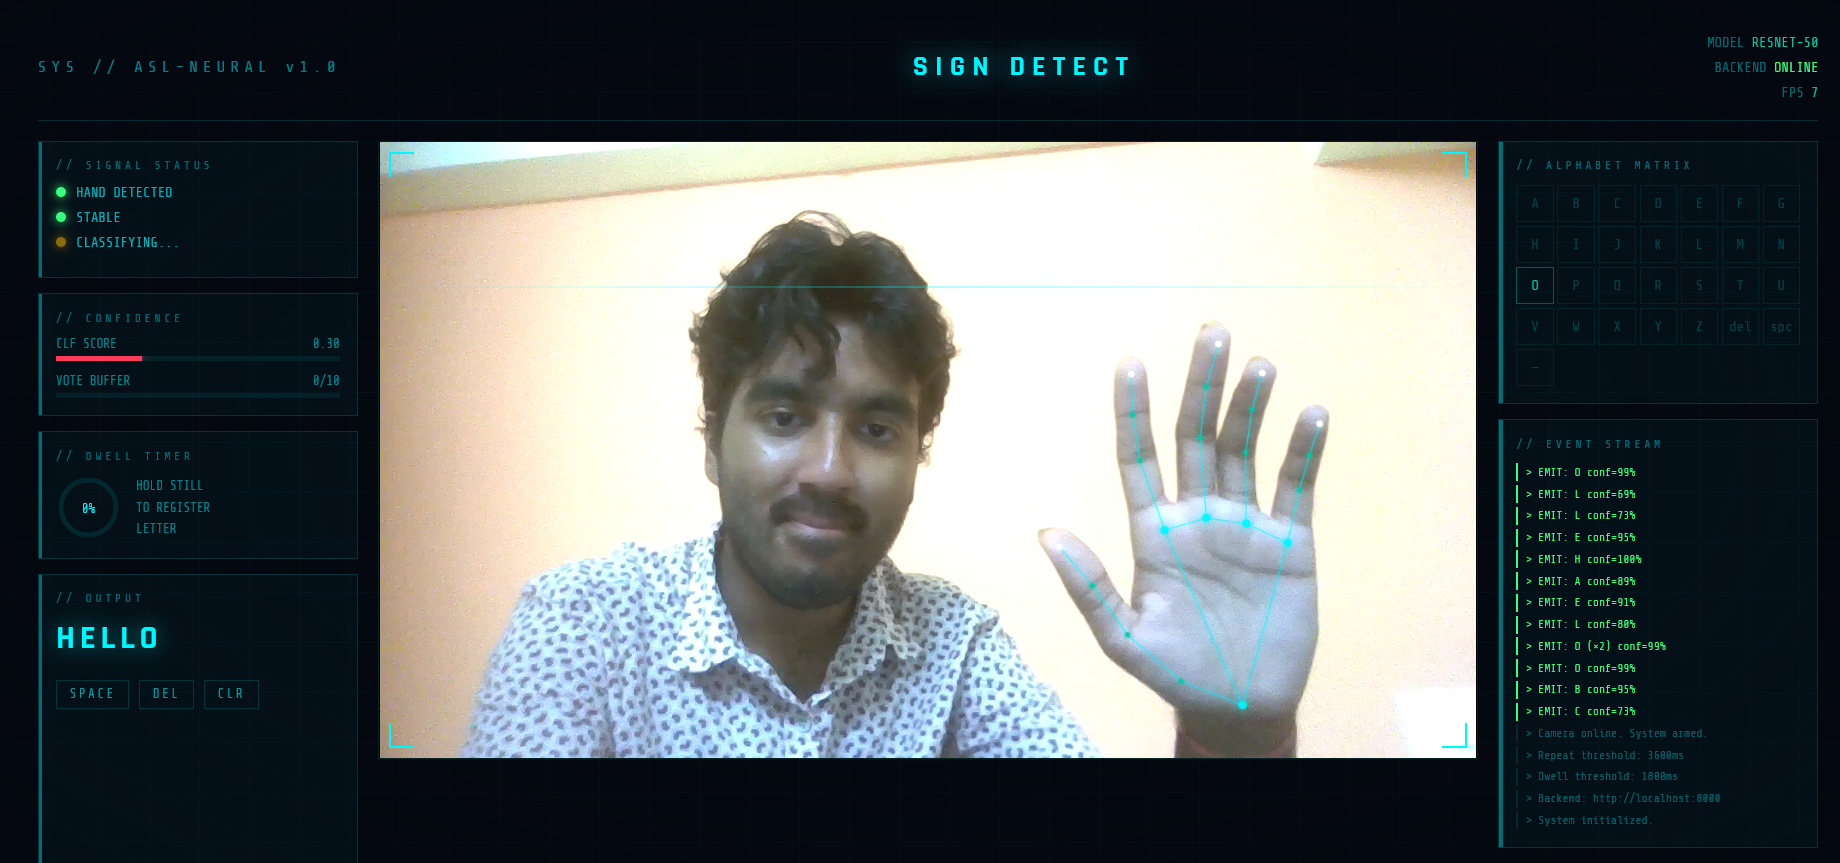
\includegraphics[width=\textwidth]{api_ss}
    \caption{FastAPI \texttt{/predict} endpoint response for a live hand frame, showing letter, confidence, bounding box, handedness, motion, and landmark fields.}
    \label{fig:api}
\end{figure*}

\subsection{Browser Frontend}

A single-page HTML/JavaScript frontend connects to the FastAPI server and provides 
real-time visual feedback. Client-side MediaPipe (via the Tasks Vision JS SDK) runs 
at 60\,fps to render the hand skeleton overlay with zero latency, while frames are 
sent to the backend at approximately 8\,fps for classification. The UI includes a 
dwell-based letter emission mechanism: a predicted letter must remain stable for 
1.8\,s before being appended to the output transcript, with subsequent repetitions 
requiring 3.6\,s. This prevents spurious emissions from brief hand holds.

% -------------------------------------------------------
\section{Results and Discussion}
\label{sec:results}

\textit{Training was conducted on a Google Colab T4 GPU. Due to session time limits 
and compute availability, fine-tuning was run for 3 epochs rather than the full 
scheduled 200. The results below reflect this constrained run.}

The model was trained for 3 epochs with batch size 128 using the SGD (Nesterov) optimizer 
and the cosine annealing schedule with linear warm-up described in Section~IV. 
Table~\ref{tab:results} summarizes the final performance metrics.

\begin{table}[h]
\caption{Training and Evaluation Results}
\label{tab:results}
\centering
\begin{tabular}{lcc}
\toprule
\textbf{Split} & \textbf{Loss} & \textbf{Accuracy (\%)} \\
\midrule
Train (epoch 3) & 0.0474 & 99.03 \\
Validation      & 0.0099 & 99.86 \\
Test            & 0.0096 & 99.80 \\
\bottomrule
\end{tabular}
\end{table}

The model reached \textbf{99.80\%} test accuracy in 3 epochs, rising from 64.41\% 
validation accuracy at epoch 1 to 99.86\% by epoch 3. Given the training was 
terminated far short of the configured maximum, these numbers are largely a 
reflection of the ImageNet-pretrained backbone's strong prior and the relatively 
constrained nature of the dataset — controlled backgrounds, consistent framing, 
single hand per image — rather than a claim of general robustness. W\&B logs 
confirmed a mean gradient norm of 1.64 and a gradient clipping ratio of 0.77 at 
the final epoch, indicating the clipping constraint was active and the optimization 
trajectory was still steep at termination. A full run to convergence would likely 
yield marginal additional gains on this dataset but would be more informative for 
harder, real-world evaluation sets.

\begin{figure*}[!t]
    \centering
    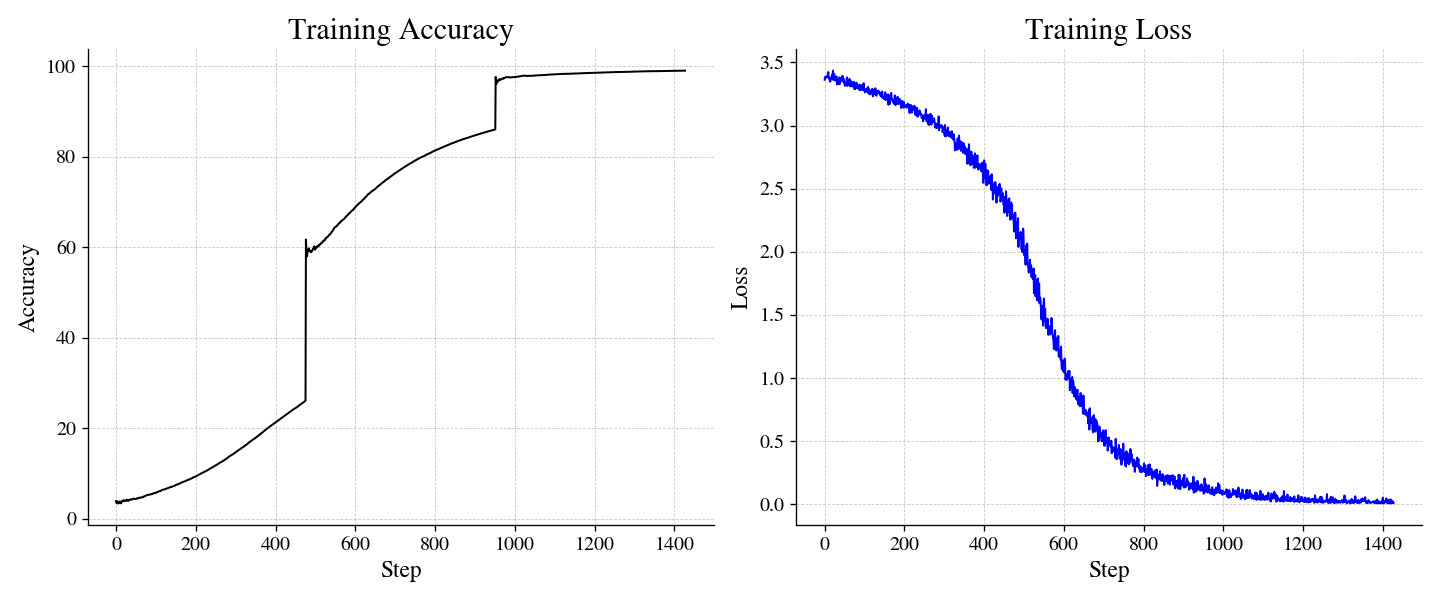
\includegraphics[width=\textwidth]{Training Plots}
    \caption{Training and validation loss/accuracy curves across epochs, logged via Weights \& Biases.}
    \label{fig:training}
\end{figure*}

The primary challenge for real-world deployment remains generalization to hand 
appearances outside the training distribution — varied skin tones, lighting 
conditions, and cluttered backgrounds not represented in the Kaggle dataset. 
The two-stage architecture mitigates this partially by isolating the classifier 
from background noise via the MediaPipe ROI crop.

% -------------------------------------------------------
\section{Conclusion}

This paper presents a real-time ASL alphabet recognition system combining MediaPipe hand detection with ResNet-50 classification. The system achieves 99.80\% test accuracy on the Kaggle ASL Alphabet dataset and operates at interactive frame rates via a FastAPI inference server and browser-based frontend. The training pipeline incorporates warm-up scheduling, Nesterov SGD, gradient clipping, and early stopping for robust convergence. A dwell-based temporal emission mechanism and majority-vote buffer ensure stable, low-noise letter output in real-time use. This work addresses a meaningful accessibility problem and establishes a practical baseline for further extensions, including full ASL word-level recognition and continuous signing.

Future directions include:
\begin{itemize}
    \item Fine-tuning MediaPipe on a dedicated hand detection dataset for improved localization accuracy.
    \item Upgrading the backbone to ResNet-152 or EfficientNet for higher classification capacity.
    \item Extending the vocabulary to dynamic gestures and full ASL words using temporal models (e.g., LSTM or Transformer-based sequence models).
    \item Deploying the system as a mobile application for broader accessibility.
\end{itemize}

% -------------------------------------------------------
\begin{thebibliography}{00}

\bibitem{who2021}
World Health Organization, ``Deafness and hearing loss,'' \textit{WHO Fact Sheets}, 2021. [Online]. Available: \url{https://www.who.int/news-room/fact-sheets/detail/deafness-and-hearing-loss}

\bibitem{redmon2016}
J. Redmon, S. Divvala, R. Girshick, and A. Farhadi, ``You only look once: Unified, real-time object detection,'' in \textit{Proc. IEEE CVPR}, 2016, pp. 779--788.

\bibitem{he2016}
K. He, X. Zhang, S. Ren, and J. Sun, ``Deep residual learning for image recognition,'' in \textit{Proc. IEEE CVPR}, 2016, pp. 770--778.

\bibitem{mitra2007}
S. Mitra and T. Acharya, ``Gesture recognition: A survey,'' \textit{IEEE Trans. Syst., Man, Cybern. C, Appl. Rev.}, vol. 37, no. 3, pp. 311--324, 2007.

\bibitem{pigou2015}
L. Pigou, S. Dieleman, P.-J. Kindermans, and B. Schrauwen, ``Sign language recognition using convolutional neural networks,'' in \textit{Proc. ECCV Workshops}, 2015.

\bibitem{kaggle_asl}
A. Akash, ``ASL Alphabet,'' Kaggle, 2018. [Online]. Available: \url{https://www.kaggle.com/datasets/grassknoted/asl-alphabet}

\bibitem{wandb}
L. Biewald, ``Experiment tracking with weights and biases,'' 2020. [Online]. Available: \url{https://www.wandb.com}

\bibitem{fastapi}
S. Ram\'irez, ``FastAPI,'' 2018. [Online]. Available: \url{https://fastapi.tiangolo.com}

\end{thebibliography}

\end{document}